\documentclass[multi=tikzpicture,border=8pt]{standalone}
\usepackage[UTF8]{ctex}
\usepackage{amsmath,amssymb,tikz}
\usetikzlibrary{arrows.meta,calc}
\definecolor{blue}{HTML}{17365D}
\definecolor{red}{HTML}{AC3931}
\tikzset{every node/.style={font=\small},arrow/.style={-{Stealth[length=2.8mm]},thick},dim/.style={|<->|,thin},box/.style={draw,rounded corners,align=center,minimum width=2.5cm,minimum height=.8cm}}
\begin{document}
\begin{tikzpicture}

\draw[blue!40,thick](0,0)circle(3.2);\draw[fill=blue!12,blue](0,0)circle(.483);\draw[red,very thick](1.3585,0)ellipse(1.8415 and 1.2437);\fill[red](-.483,0)circle(3pt)node[left]{第一脉冲};\fill[red](3.2,0)circle(3pt)node[right]{第二脉冲};\draw[arrow,red](-.483,0)--(-.483,-1.4)node[left]{$v_1$};\draw[arrow,red](3.2,0)--(3.2,1.4)node[right]{$v_a$};\draw[arrow,blue](3.55,0)--(3.55,2.1)node[right]{$v_c$};\node[below]at(0,-3.8){地球位于椭圆的一个焦点；按半径比例绘制};

\end{tikzpicture}
\begin{tikzpicture}

\node[above]at(-2,2.6){地表};\draw[arrow](-2,0)--(-2,1.7)node[above]{$v_1$};\draw[thick](-3.4,0)--(-.6,0);\node[below]at(-2,-.4){最优径向分量为零};\node[above]at(3,2.6){同步半径};\draw[arrow,blue](3,0)--(3,1.2)node[right]{$v_a$};\draw[arrow,red](3,1.2)--(3,2.2)node[right]{$\Delta v_2$};\draw[arrow](2.2,0)--(2.2,2.2)node[left]{$v_c$};\node[below]at(3,-.4){$\Delta v_2=v_c-v_a$};

\end{tikzpicture}
\begin{tikzpicture}
\draw[arrow](0,0)--(6.3,0)node[right]{$w/(\mathrm{km/s})$};\draw[arrow](0,0)--(0,5.3)node[above]{$C/(\mathrm{km/s})$};\draw[very thick,blue] plot coordinates {(0.00000,1.18329) (0.02010,1.17827) (0.04020,1.17325) (0.06030,1.16824) (0.08040,1.16323) (0.10050,1.15823) (0.12060,1.15323) (0.14070,1.14824) (0.16080,1.14325) (0.18090,1.13827) (0.20101,1.13329) (0.22111,1.12831) (0.24121,1.12334) (0.26131,1.11838) (0.28141,1.11342) (0.30151,1.10847) (0.32161,1.10352) (0.34171,1.09857) (0.36181,1.09364) (0.38191,1.08870) (0.40201,1.08377) (0.42211,1.07885) (0.44221,1.07393) (0.46231,1.06901) (0.48241,1.06410) (0.50251,1.05920) (0.52261,1.05430) (0.54271,1.04940) (0.56281,1.04451) (0.58291,1.03963) (0.60302,1.03475) (0.62312,1.02987) (0.64322,1.02500) (0.66332,1.02013) (0.68342,1.01527) (0.70352,1.01042) (0.72362,1.00557) (0.74372,1.00072) (0.76382,0.99588) (0.78392,0.99104) (0.80402,0.98621) (0.82412,0.98138) (0.84422,0.97656) (0.86432,0.97175) (0.88442,0.96693) (0.90452,0.96213) (0.92462,0.95732) (0.94472,0.95253) (0.96482,0.94773) (0.98492,0.94295) (1.00503,0.93816) (1.02513,0.93339) (1.04523,0.92861) (1.06533,0.92385) (1.08543,0.91908) (1.10553,0.91432) (1.12563,0.90957) (1.14573,0.90482) (1.16583,0.90008) (1.18593,0.89534) (1.20603,0.89061) (1.22613,0.88588) (1.24623,0.88115) (1.26633,0.87643) (1.28643,0.87172) (1.30653,0.86701) (1.32663,0.86231) (1.34673,0.85761) (1.36683,0.85291) (1.38693,0.84822) (1.40704,0.84354) (1.42714,0.83886) (1.44724,0.83418) (1.46734,0.82951) (1.48744,0.82485) (1.50754,0.82019) (1.52764,0.81553) (1.54774,0.81088) (1.56784,0.80623) (1.58794,0.80159) (1.60804,0.79695) (1.62814,0.79232) (1.64824,0.78770) (1.66834,0.78307) (1.68844,0.77846) (1.70854,0.77385) (1.72864,0.76924) (1.74874,0.76464) (1.76884,0.76004) (1.78894,0.75545) (1.80905,0.75086) (1.82915,0.74628) (1.84925,0.74170) (1.86935,0.73712) (1.88945,0.73256) (1.90955,0.72799) (1.92965,0.72343) (1.94975,0.71888) (1.96985,0.71433) (1.98995,0.70979) (2.01005,0.70525) (2.03015,0.70071) (2.05025,0.69618) (2.07035,0.69166) (2.09045,0.68714) (2.11055,0.68262) (2.13065,0.67811) (2.15075,0.67361) (2.17085,0.66911) (2.19095,0.66461) (2.21106,0.66012) (2.23116,0.65563) (2.25126,0.65115) (2.27136,0.64667) (2.29146,0.64220) (2.31156,0.63774) (2.33166,0.63327) (2.35176,0.62882) (2.37186,0.62436) (2.39196,0.61992) (2.41206,0.61547) (2.43216,0.61103) (2.45226,0.60660) (2.47236,0.60217) (2.49246,0.59775) (2.51256,0.59333) (2.53266,0.58892) (2.55276,0.58451) (2.57286,0.58010) (2.59296,0.57570) (2.61307,0.57131) (2.63317,0.56692) (2.65327,0.56253) (2.67337,0.55815) (2.69347,0.55377) (2.71357,0.54940) (2.73367,0.54504) (2.75377,0.54068) (2.77387,0.53632) (2.79397,0.53197) (2.81407,0.52762) (2.83417,0.52328) (2.85427,0.51894) (2.87437,0.51461) (2.89447,0.51028) (2.91457,0.50596) (2.93467,0.50164) (2.95477,0.49732) (2.97487,0.49301) (2.99497,0.48871) (3.01508,0.48441) (3.03518,0.48012) (3.05528,0.47583) (3.07538,0.47154) (3.09548,0.46726) (3.11558,0.46298) (3.13568,0.45871) (3.15578,0.59454) (3.17588,0.80264) (3.19598,0.98630) (3.21608,1.15384) (3.23618,1.30977) (3.25628,1.45680) (3.27638,1.59677) (3.29648,1.73095) (3.31658,1.86027) (3.33668,1.98546) (3.35678,2.10706) (3.37688,2.22553) (3.39698,2.34123) (3.41709,2.45445) (3.43719,2.56545) (3.45729,2.67443) (3.47739,2.78158) (3.49749,2.88706) (3.51759,2.99100) (3.53769,3.09351) (3.55779,3.19472) (3.57789,3.29470) (3.59799,3.39355) (3.61809,3.49133) (3.63819,3.58811) (3.65829,3.68396) (3.67839,3.77893) (3.69849,3.87307) (3.71859,3.96643) (3.73869,4.05904) (3.75879,4.15095) (3.77889,4.24219) (3.79899,4.33280) (3.81910,4.42280) (3.83920,4.51223) (3.85930,4.60110) (3.87940,4.68945) (3.89950,4.77729) (3.91960,4.86466) (3.93970,4.95156) (3.95980,5.03801) (3.97990,5.12404) (4.00000,5.20967)};\fill[red](3.14419,.45691)circle(3pt);\draw[dashed](3.14419,0)--(3.14419,.45691);\node[below]at(3.14419,0){1.57210};\node[left]at(0,.45691){11.91381};\node[left]at(0,2){15};\node[above]at(3,6.1){左段递减，右段递增，分界点最优};
\end{tikzpicture}
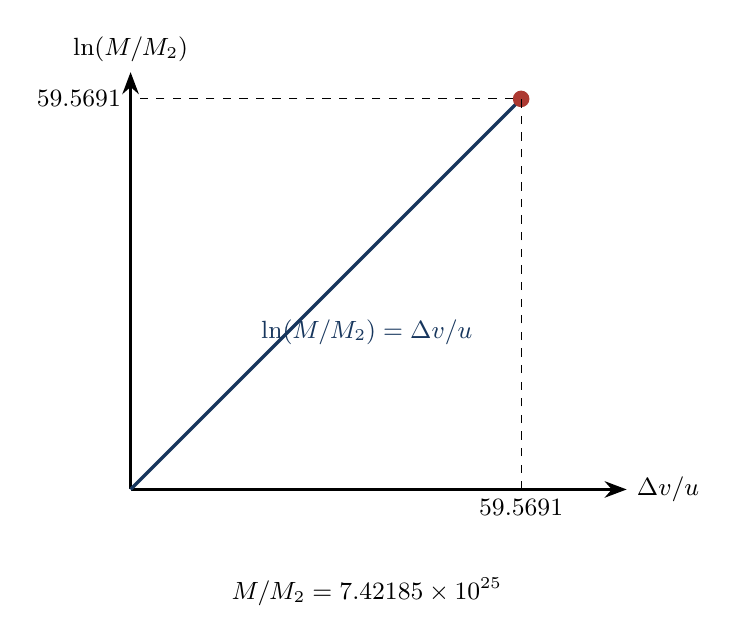
\begin{tikzpicture}
\draw[arrow](0,0)--(6.3,0)node[right]{$\Delta v/u$};\draw[arrow](0,0)--(0,5.3)node[above]{$\ln(M/M_2)$};\draw[blue,very thick](0,0)--(5,5);\fill[red](4.96,4.96)circle(3pt);\draw[dashed](4.96,0)--(4.96,4.96)--(0,4.96);\node[below]at(4.96,0){59.5691};\node[left]at(0,4.96){59.5691};\node[blue]at(3,2){$\ln(M/M_2)=\Delta v/u$};\node[below]at(3,-1){$M/M_2=7.42185\times10^{25}$};
\end{tikzpicture}
\begin{tikzpicture}

\node[box](a)at(0,0){能量守恒\\确定地表速率};\node[box](b)at(5,0){角动量守恒\\约束到达$v_r,w$};\node[box,fill=blue!8](c)at(2.5,-2){最小矢量增量和\\两端均为切向速度};\draw[arrow](a)--(c);\draw[arrow](b)--(c);\node[below]at(2.5,-3.2){地表静止初态：第一增量等于完整$v_1$};

\end{tikzpicture}
\end{document}
